%        File: cahier_des_charges.tex
%     Created: sam. oct. 22 06:00  2016 C
% Last Change: sam. oct. 22 06:00  2016 C
%
\documentclass[a4paper]{article}
\usepackage[francais]{babel}
\usepackage[T1]{fontenc}
\usepackage[utf8]{inputenc}
\usepackage{graphicx}

\frenchspacing
\author{KostiTeam}
\title{Cahier des charges}

\setcounter{secnumdepth}{4}

\begin{document}

\maketitle
\newpage
\tableofcontents
\newpage

\section{Probl\'ematique}
La virtualisation est le fait de cr\'eer une version virtuelle d'une entit\'e physique, ces versions virtuelles
sont alors appel\'ees Machines virtuelles ou VM (Virtual Machine). Nous pouvons prendre comme exemple Virtual
Box, qui est un outil de virtualisation permettant d'\'emuler un syst\`eme d'exploitation (linux ou autre).
Les diff\'erentes ressources de la machine h\^ote sont alors partag\'ees et allou\'ees dynamiquement aux
diff\'erentes machines virtuelles par des logiciels appel\'es hyperviseur.\\

La virtualisation peut \^etre utile dans diverses situations. En effet, virtualiser un environnement/un objet 
permet de trouver ses caract\'eristiques optimales \`a moindre co\^ut. De plus, cela permet aussi d'acqu\'erir
des comp\'etences sans pour autant disposer de mat\'eriel. Dans le cadre d'\'etudes informatiques, il peut
\^etre pratique de simuler des r\'eseaux dans lesquels des machines dialoguent. Marionnet est un exemple de
logiciel de simulation de r\'eseaux. Cependant, apr\`es l'avoir utiliser un tant soit peu, il s'av\`ere que
plusieurs d\'efauts g\^enent son utilisation : 
\begin{itemize}
  \item crashs assez fr\'equents;
  \item impossible de changer les configurations des machines en marche;
  \item processus d'arr\^et des machines trop fastidieux;
  \item interface peu ergonomique;
  \item logiciel trop gourmand en ressources.
\end{itemize}


Face \'a ces probl\`emes, nous avons donc d\'ecid\'e de cr\'eer un nouveau simulateur de r\'eseaux.

\section{Solution}
Pour pallier les probl\`emes expos\'es pr\'ecedemment, il nous semble pertinent de ne pas virtualiser les
machines utilis\'ees  (VM) mais uniquement les environnements (VE).\\

Les VM ont un d\'efaut pour nous: elles simulent tout le materiel d'une machine (processeur, RAM...).
Nous prefererons donc utiliser des VE (Virtual Environement). Les VE permetttent de ne simuler que le
systeme d'exploitation, et de partager le m\^eme noyeau qu la machine h\^ote, et donc, de r\'epartir les
ressources entre machine h\^ote et les differents environements virtuels. Cette solution correspondrait donc
plus a nos besoins, grace a un gain notable de performance, notamment lorsque le nombre de machines est
important.\\

Pour virtualiser les environnements, nous avons choisi d'utiliser la technologie de LXC.

\section{LXC}
\subsection{D\'efinition}

LXC est un outil de virtualisation permettant de cr\'eer des environnements virtuels, diff\'erents systemes
d'exploitations sont mis a disposition (Ubuntu, Debian...). Ces Environnements sont appel\'ees containers. Le
partage des ressources est assur\'e par l'outil Cgroups du noyau, qui permet de limiter, compter et
isoler l'utilisation des ressources.\\

Chaque environnement virtuel est isol\'ee, de la m\^eme mani\`ere que l'isolement d'un programme 
avec "\emph{chroot}": chaque environnement est cr\'e\'e de mani\`ere \`a ce qu'ils naient pas acc\`es au syst\`eme 
d'exploitation de la machine h\^ote. En revanche, la machine h\^ote, elle, a acc\`es aux machines virtuelles.
Cette isolation entre les machines virtuelles et la machine h\^ote, permet de garantir une certaine s\'ecurit\'e.\\

\subsection{Pourquoi LXC ?}

LXC poss\`ede sa propre API, notamment en C/C++, ce qui nous permet de l'int\'egrer ) notre projet efficacement.
Il est plus l\'eger que des technologies comme Docker (qui h\'erite de LXC) et convient \`a notre utilisation.

\subsection{Fonctionnement de LXC}

\subsubsection{Les containers, leur fonctionnement}

Les environnements virtuels, ou, containers (conteneurs en francais)  doivent, en premier temps, \^etre cr\'e\'es
\`a l'aide de la commande "\emph{lxc-create ...}" (voir notices pour plus de pr\'ecisions sur les commandes). De
nombreux syst\`emes d'exploitation seront alors propos\'es, (nous avons choisi de prendre Debian, Jessie,
i386). Par d\'efaut, les machines cr\'e\'ees ne sont pas configur\'ees: elles n'ont pas d'interfaces, elles 
n'ont pas de compilateur, et les utilitaires pr\'einstall\'es sont tr\`es rudimentaire 
(pas de ping, ifconfig, tcpdump...).\\

Chaque container poss\`ede un fichier de configuration situ\'e \`a l'emplacement suivant: "\emph{/var/lib/lxc/<nom 
du container>/config}". Il est possible de configurer de nombreux aspect du container dans ce fichier 
(par exemple: modifier les variables d'environnement, ou changer le nom d'h\^ote ("\emph{hostname}") du 
container. Voir "\emph{man lxc}" pour en savoir plus). Ce fichier va notamment permettre de param\'etrer la 
configuration r\'eseau du container \`a son d\'emarrage (c'est ce qui va nous int\'eresser en priorit\'e avec 
ce fichier).\\

Les containers se lancent avec la commande "\emph{lxc-start ...}"; il est pr\'ef\'erable de les lancer en d\'emons
(en arri\`ere-plan), puis d'y "\emph{attacher}" un terminal avec "\emph{lxc-attach}", afin d'\^etre connect\'e
en super utilisateur (ou root) car, premi\`erement, par d\'efaut, aucun profil d'utilisateur n'est cr\'e\'e sur 
le container, et, de plus, cela permet d'avoir l'entier contr\^ole du container afin de, par exemple, modifier 
son adresse ipv4.\\


\subsubsection{Bridges et fonctionnement r\'eseau}
\paragraph{fichier de configuration}~\\

Comme expliqu\'e plus haut, les param\`etres r\'eseaux du container peuvent \^etre modifi\'es via le fichier config.
Dans ce fichier, chaque "\emph{block}" permet de d\'efinir une interface. Un block commence toujours par la 
d\'efinition du type de r\'eseau, nous allons donc nous int\'eresser tout d'abord au type de r\'eseau
("\emph{lxc.network.type}").
Plusieurs types de r\'eseaux sont disponibles, mais, nous allons choisir le type veth, qui signifie Virtual 
Ethernet, ce type permet d'\'etablir un lien entre l'interface virtuelle du container et un pont, pr\'ealablement
cr\'e\'e sur la machine host (nous verrons cette liaison plus en d\'etail par la suite).\\

Ce fichier permet aussi d'\'etablir des adresses ipv4 ("\emph{lxc.network.ipv4}"), ipv6 ("\emph{lxc.network.ipv6}"),
et mac ("\emph{lxc.network.hwaddr}"), ainsi que leurs Broadcast. Cela permet de mettre en place le r\'eseau 
virtuel avant de lancer les machines; bien que ces param\`etres puissent \^etre modifi\'es une fois la machine
lanc\'ee \`a l'aide de l'outil "\emph{ifconfig}". Attention, les tables de routage ne peuvent pas \^etre
configur\'ees d'avance, il faut les configurer une fois le VE lanc\'e.\\

Le dernier param\`etre que nous verrons pour ce fichier est le lien ("\emph{lxc.network.link}"); ce param\`etre
va permettre d'indiquer \`a quel bridge nous voulons connecter notre interface.\\

\paragraph{Bridges}~\\

Les bridges (ou pont en francais) sont des \'equipements r\'eseaux qui permettent de relier deux (ou plus)
interfaces de mani\`ere compl\`etement transparente: en observant les paquets qui transitent, le pont peut 
connaitre les adresses mac des interfaces, et ainsi, rediriger les paquets. Les ponts peuvent par exemple,
\^etre utilis\'es pour rediriger une connexion Ethernet: une machine se connecte en Ethernet, une seconde 
machine se connecte \`a la premi\`ere, elles \'etablissent un pont entre deux de leurs interfaces (une interface
de la premi\`ere machine, et une interface de la deuxi\`eme machine), et, ainsi, la deuxi\`eme machine peut 
avoir acc\`es \`a internet.\\

Lorsqu'un VE se lance, une interface se cr\'e\'e sur la machine h\^ote pour chaque interface pr\'esente sur le VE.
Ces interfaces cr\'e\'ees ont un noms qui commencent toujours par "\emph{VETH}" suivit de quatre caract\`eres. Ces
interfaces sur la machine h\^ote representent les interfaces de l'environement virtuels, et vons nous permettre des
reliers les environnements entre eux; il est possible de voir la correspondance entre les interfaces d'un container
et les interfaces de la machine h\^ote grace a la commande "\emph{lxc-info ...}".\\

Il est donc necessaire de relier ces interfaces sur la machine h\^ote a un m\^eme bridge pour que les 
containers puissent communiquer!

\newpage
\section{Architecture du programme}
\subsection{Vues}
Le logiciel a une seule interface : 
\begin{center}
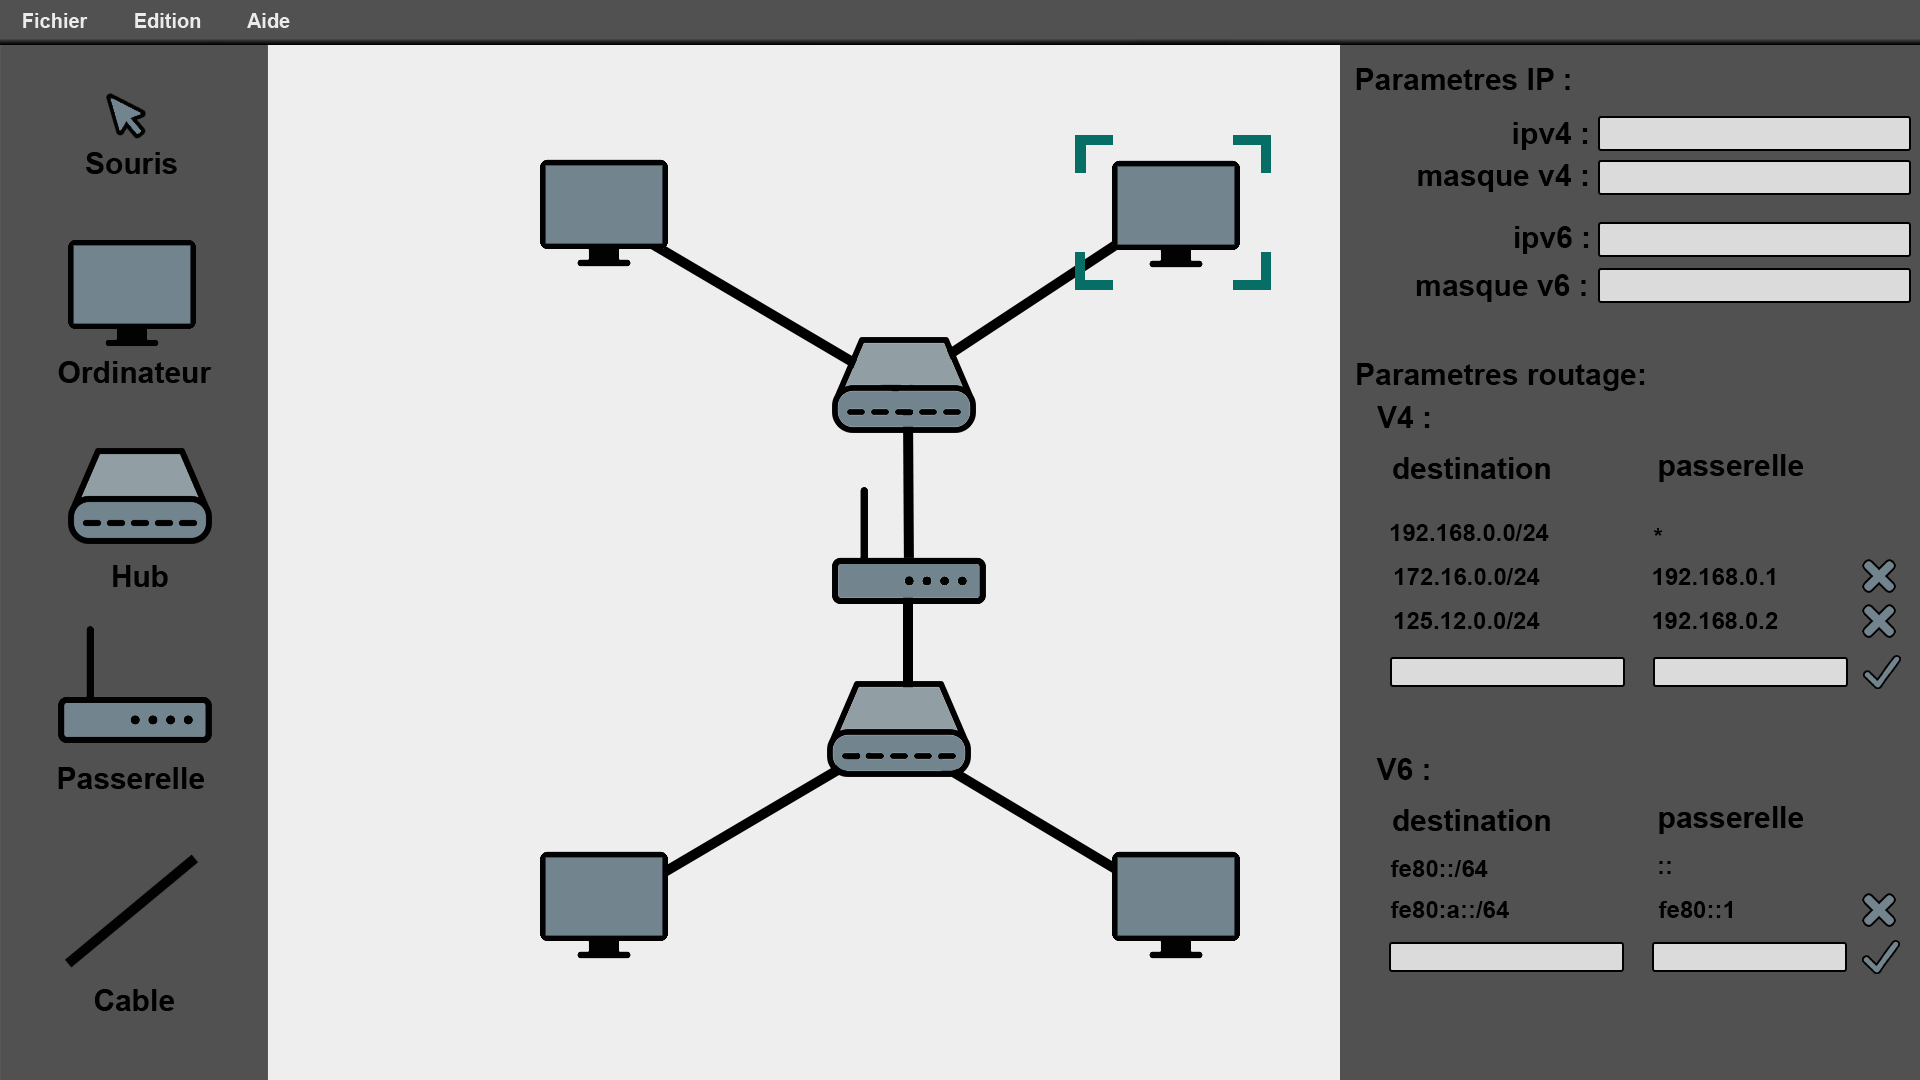
\includegraphics[scale=0.2]{bulto.png}
\end{center}

Elle est divisible en 4 parties : 
\begin{itemize}
\item La barre supérieure (Fichier, Éditions, Aide...),
\item la barre de sélection (à gauche) où on peut choisir quel entité ajouter,
\item l'écran principal (au centre),
\item la barre d'information (à droite) où sont affichées les configurations des entités sélectionnées.
\end{itemize}

\subsection{Diagrammes}


\section{Etapes pr\'evues}


\section{Notice d'utilisation de LXC}

\documentclass[twoside]{article}
\usepackage[francais]{babel}
\usepackage[T1]{fontenc}
\frenchspacing
\author{KostiTeam}
\title{Manuel d'utilisation LXC}
\begin{document}

\maketitle
\newpage
\tableofcontents
\newpage

\section{Bien d\'ebuter}
Toutes les commandes ex\'ecut\'ees sont effectu\'ees en root (super-utilisateur).

\subsection{Installer LXC}
\subsubsection{Arch-linux}
\emph{\#pacman -S lxc arch-install-scripts}
\subsubsection{Debian}
\emph{\#apt-get install lxc}

\subsection{Cr\'eer un container}
\emph{\#lxc-create -t download -n name}: cr\'eer un container de nom name en proposant la liste des images d'OS possibles \`a t\'el\'echarger.\\ 

\emph{\#lxc-create -t download -n name -d debian -r jessie -a i386}: cr\'eer un container de nom \emph{name} en t\'el\'echargeant une image de distribution \emph{debian}, de release \emph{jessie} et d'architecture \emph{i386} (32 bits).\footnote{Cr\'eer un container d'architecture 64 bits sur un host 32 bits \textbf{ne fonctionne pas}.}\\

\emph{\#lxc-ls}: obtenir la liste des containers cr\'e\'es --fancy pour plus de d\'etails.\\
  
\subsection{D\'emarrer un container}
\emph{\#lxc-start -n name  -d}: d\'emarrer le container de nom \emph{name} en daemon \emph{(-d)}.\\
Par d\'efaut, aucun compte utilisateur n'est cr\'e\'e. Il faut donc se connecter en root.\\ 

\emph{\#lxc-attach -n name}: se connecter en root sur le container \emph{name}.\\
Une fois un compte utilisateur cr\'e\'e, il est possible de lancer un terminal sur une session.\\

\emph{\#lxc-console -n name -t 0}: ouvrir un \'ecran de login sur le terminal tty0 du container \emph{name}.\footnote{\textbf{BUG:} sur certaines distributions, -t diff\'erent de 0 ne fonctionne pas}\\

\subsection{Configurer un container}
\subsubsection{Fichier de configuration}
Le fichier de configuration d'un container \emph{name} est /var/lib/lxc/\emph{name}/config. Voici un exemple de configuration de passerelle:\\
\emph{RTFM: lxc.container.conf}\\

\noindent
\textbf{/var/lib/lxc/passerelle/config}\\

\noindent
\# Distribution configuration\\
lxc.include = /usr/share/lxc/config/debian.common.conf\\
lxc.arch = x86\_64\\

\noindent
\# Container specific configuration\\
lxc.rootfs = /var/lib/lxc/passerelle/rootfs\\
lxc.rootfs.backend = dir\\
lxc.utsname = passerelle\\

\noindent
\# Network configuration\\
lxc.network.type = veth\\
lxc.network.name = eth0\\
lxc.network.link = lxcbr0\\
lxc.network.flags = up\\
lxc.network.hwaddr = 00:16:3e:5b:0e:8f\\
lxc.network.ipv4 = 172.16.1.1\\
lxc.network.ipv6 = fec00:0:0:2::1\\

\noindent
lxc.network.type = veth\\
lxc.network.name = eth1\\
lxc.network.link = lxcbr0\\
lxc.network.flags = up\\
lxc.network.hwaddr = 00:16:3e:5b:0e:8f\\
lxc.network.ipv4 = 192.168.1.1\\
lxc.network.ipv6 = fc00:0:0:1::1\\

Ici, le container poss\`ede deux interfaces (eth0 et eth1) avec chacune leurs adresses ipv4 (lxc.network.ipv4),
ipv6 (lxc.network.ipv6) et MAC (hwaddr).\\
lxc.network.flags indique quelle action effectuer (up active l'interface).\\
lxc.network.type indique quelle type de virtualisation de réseau utiliser (RTFM).\\
lxc.network.link indique l'interface \`a utiliser pour le vrai trafic, cette notion sera vu plus en d\'etail par la suite.\\

\subsubsection{ifconfig, ip}

***Commandes ip/ifconfig pour ipv4,ipv6***

\subsection{Relier les containers}
\subsubsection{Les Bridges -- Ponts}

Pour relier les containers entre eux, ou m\^eme au host, LXC utilise les bridge (pont en francais). Lors de
la cr\'eation d'un container, l'activation de chacune de ses interfaces va cr\'eer une interface sur la machine
host. Relier ces interfaces \`a un m\^eme pont permet de relier les containers "physiquement".\\

\noindent
\emph{\#brctl addbr br0}: cr\'ee un bridge de nom \emph{br0}\\
\emph{\#ifconfig br0 up}: active l'interface \emph{br0}



\end{document}


\section{Rapport de bug}

\end{document}


